\chapter{Napájecí systém vesty}
Napájecí systém vesty má za úkol poskytovat elektrický výkon v požadované kvalitě, pro správnou funkci dalších obvodů ve vestě.

Hlavním zdrojem energie vesty je lithium-polymerový akumulátorem 2XLP7836140, s kapacitou 7600~\jedn{mAh}, který by měl zajistit dostatečnou výdrž vesty. Akumulátor je vybaven ochrannými obvody proti podvibití pod hranici 2,75~\jedn{V} a přebití přes 4,30~\jedn{V}.

Úbytky napětí na modré, zelené LED 3,4~\jedn{V} a úbytkům vznikajících na spínacích prvcích při regulování jasu LED, dosahují větší hodnoty než je napětí akumulátoru. Proto bylo nutné navrhnout napájecí systém založený na zvyšujícím měniči, který zvýší napětí akumulátoru.

Další úkolem napájecího systému je zajistit nabíjení akumulátoru a sledování stavu akumulátoru.

\section{Zvyšující měnič}
\begin{figure}[H]
    \begin{center}
        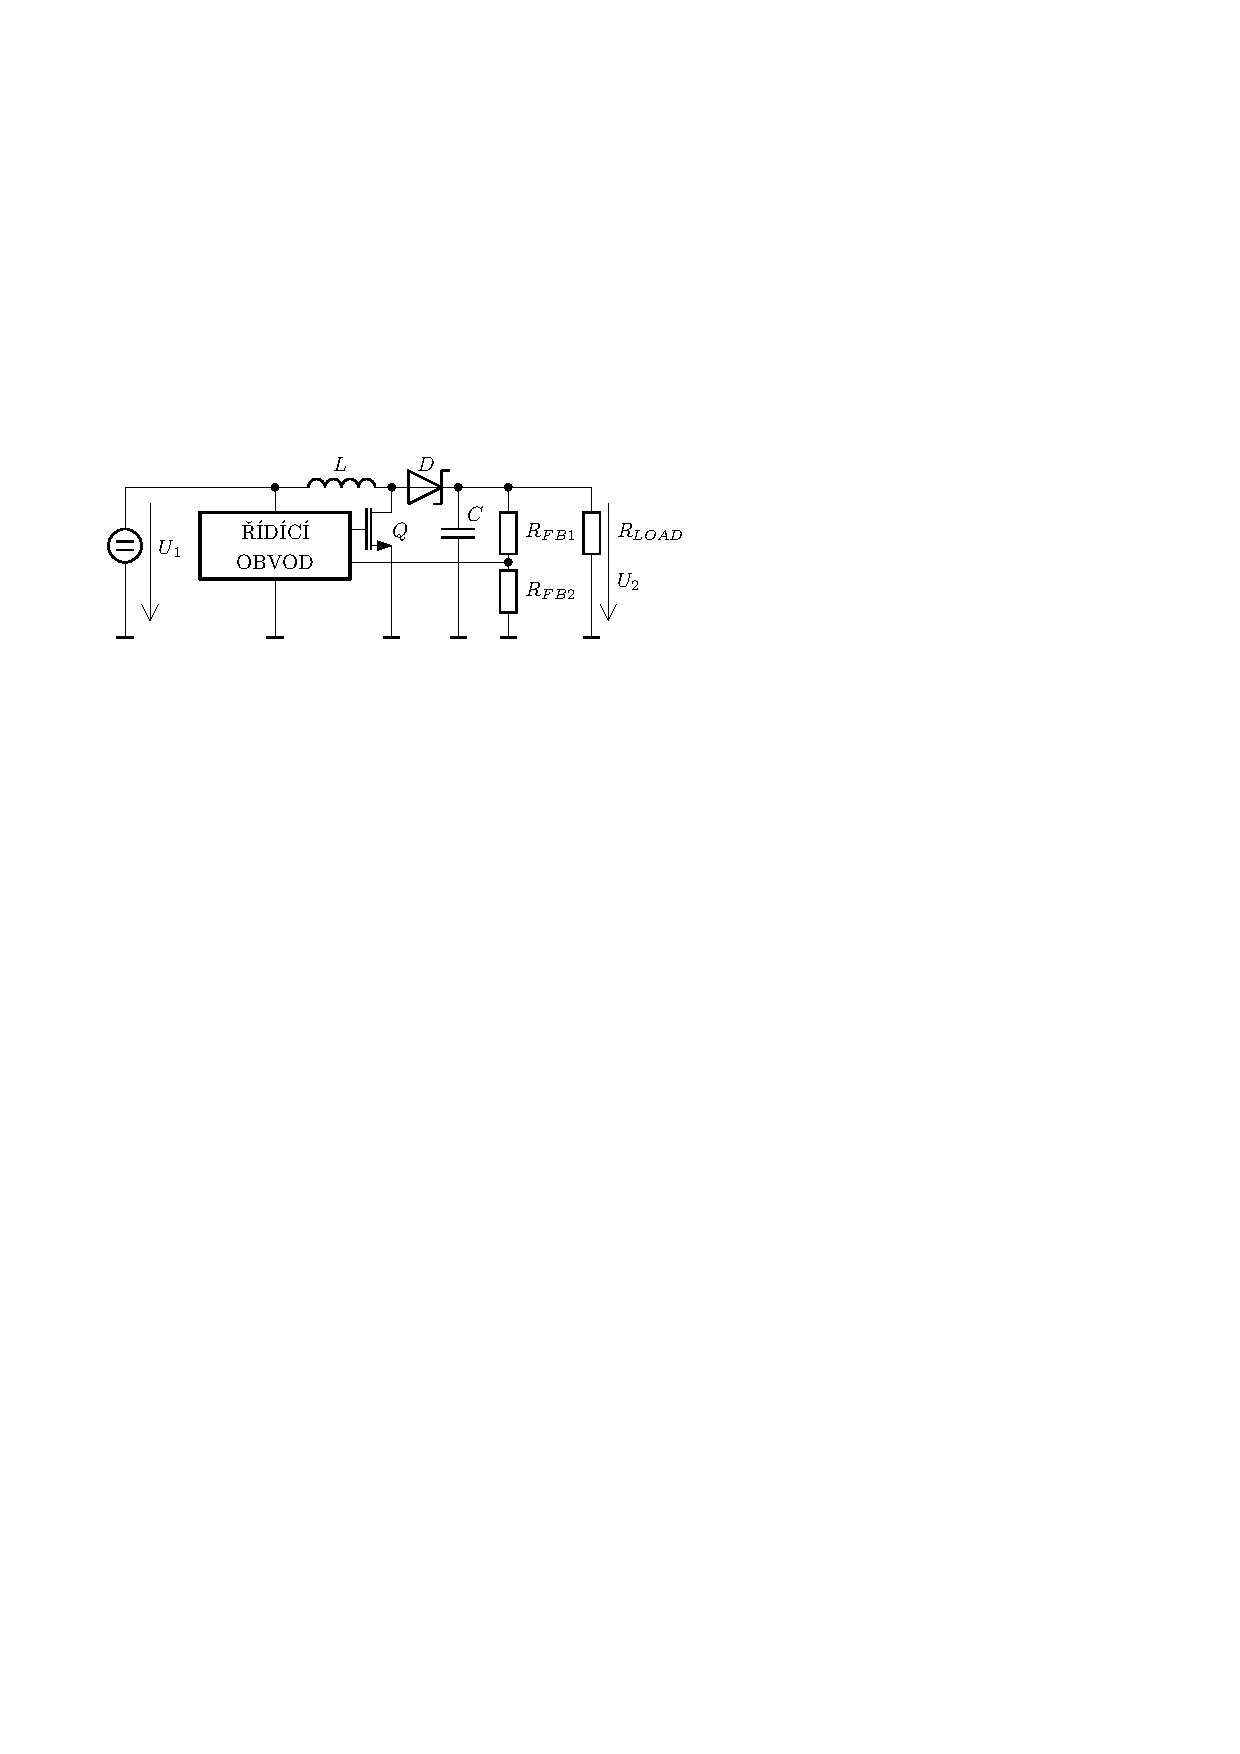
\includegraphics[width=\textwidth]{img/boost}
    \end{center}
    \caption{blokové schéma zvyšujícího měniče}
\end{figure}
Zvyšující měnič, někdy také označovaný jako boost či step up je elektrický obvod, patřící do kategorie spínaných měničů, který z vysokou účinností transformuje vstupní napětí $U_1$ na větší napětí $U_2$. Účinnost spínaných měničů dosahuje až 99~\jedn{\%}, ztráty jsou způsobeny především přeměnou části transformované elektrické energie v teplo na spínacích prvcích a ohmickém odporu vinutí cívky. Účinnost se dá zvětšit použitím měniče, který místo diody používá tranzistor. Vstupní i výstupní napětí měniče jsou stejnosměrná.

Měnič obsahuje dva akumulační prvky $L$ a $C$, které slouží k uchování energie a dva prvky aktivní $Q$ a $D$, které plní funkci spínačů. Rezistor $R_{LOAD}$ představuje zátěž.

Pokud je sepnut tranzistor, tak cívka začne akumulovat energii. V tento okamžik je dioda uzavřena, protože napětí na anodě má podprahovou hodnotu. Jakmile dojde k uzavření tranzistoru, tak se otevře dioda a začne se přesouvat akumulovaná energie z cívky do kondenzátoru.

Odvození výstupního napětí zvyšujícího měniče pro ideální spínací prvky:
\begin{eqnarray}
    i_L(t) &=& \dfrac{1}{L} \int u_L(t) \mathrm{d}t \Rightarrow u_L(t) = L \dfrac{\mathrm{d}i_L(t)}{\mathrm{d}t}
    \nonumber\\
    \dfrac{U_1 \cdot t_{ON}}{L} &=& \dfrac{(U_2 - U_1) t_{OFF}}{L} \Rightarrow U_1 \cdot t_{ON} = (U_2 - U_1) t_{OFF}
    \nonumber\\
    U_1 \cdot t_{ON} &=& U_2 \cdot t_{OFF} - U_1 \cdot t_{OFF} \Rightarrow U_1 \cdot T = U_2 \cdot t_{OFF}
    \nonumber\\
    U_2 &=& U_1 \dfrac{T}{t_{OFF}} = \underline{\underline{U_1 \dfrac{1}{1-s}}}
    \nonumber
\end{eqnarray}

Kde $t_{OFF}$ je čas po který je tranzistor sepnut, $t_{OFF}$ čas po který je tranzistor rozepnut, $T$ je perioda spínání a $s$ střída spínání.

Ze vztahu je vidět, že napětí $U_2 \geq U_1$. Pokud použijeme reálné součástky, tak tato rovnost neplatí pokud je tranzistor trvale rozepnut, tak napětí $U_2$ bude menší o úbytek na diodě a cívce. Dále ze vztahu vyplývá, že velikost výstupního napětí je závislá jen na velikosti vstupního napětí a střídě spínání.

Řídící obvod se snaží udržovat konstantní výstupní napětí, pomocí regulování střídy. Výstupní napětí je monitorováno pomocí zpětné vazby realizované napěťovým děličem. Poměr rezistorů $R_{FB1}$ a $R_{RB2}$ určuje výstupní napětí.

\section{Nabíječka}
Nabíječka zajišťuje přesouvání energie z externího zdroje do akumulátoru. Díky ní jsou akumulátory opakovatelně použitelné. Pro laser game arény je důležité, aby nabíječka byla schopná přes noc (12 hodin času) dobýt akumulátory. Vezmu-li v úvahu kapacitu akumulátoru a čas potřebný pro jeho nabitý zjistím, že nabíječka musí být schopna nabíjet akumulátor minimálně proudem 633~\jedn{mA}, od toho se odvíjel i výběr nabíjecího obvodu. Nakonec byl vybrán obvod BQ24192 od firmy Texas Instruments.

BQ24192 je určený k nabíjení lithium-iontových a lithium-polymerových akumulátorů. Je založen na snižujícím spínaném měniči, dokáže pracovat od 3,9~\jedn{V} až 17~\jedn{V} napájecí napětí a dokáže nabíjet proudem až 4,5~\jedn{A}. Dokáže monitorovat teplotu článku pomocí termistoru. Z okolím může komunikovat prostřednictvím I2C sběrnice, který umožňuje i nastavovat některé nabíjecí parametry.

\begin{figure}[H]
    \begin{center}
        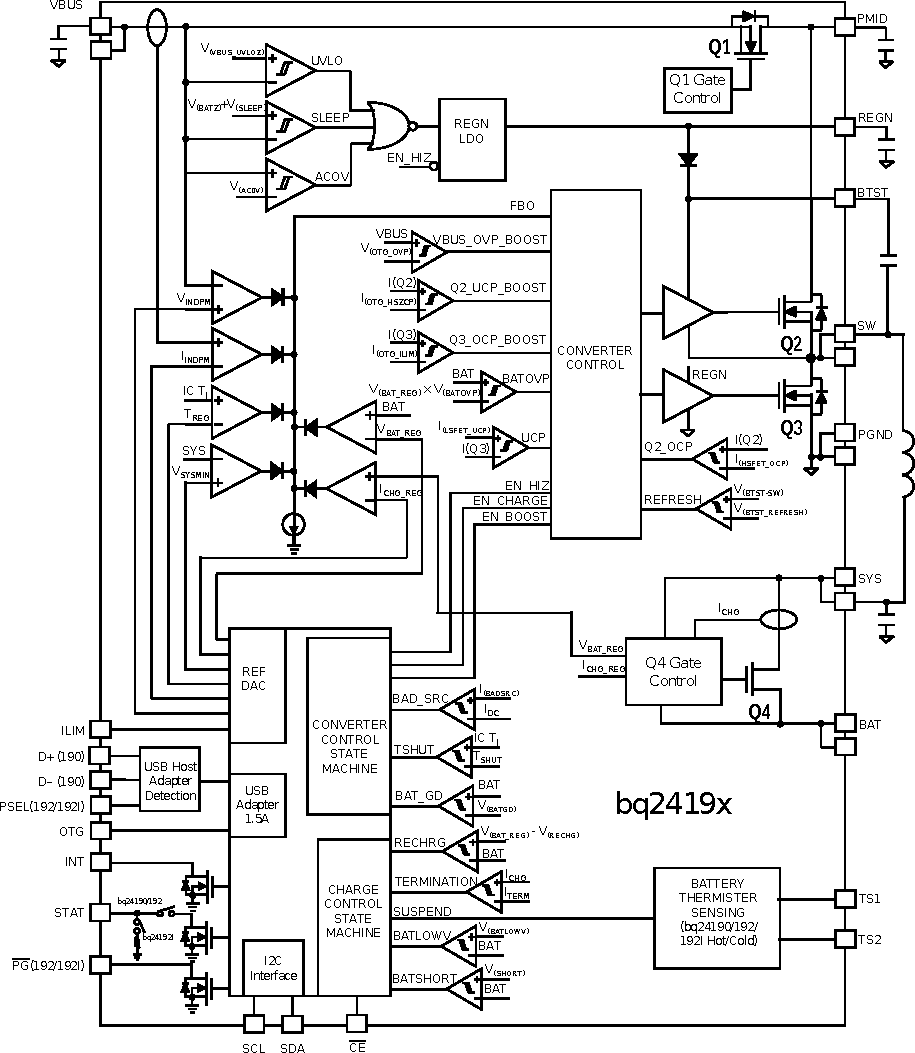
\includegraphics[width=\textwidth]{img/bq24192-block}
    \end{center}
    \caption{nabíjecí obvod BQ24192, převzato z katalogového listu výrobce}
\end{figure}

Pinem PSEL se nastaví jestli je obvod napájen z USB (vysoká úroveň) a nebo adaptéru (nízká úroveň). \Overline{CE}~ povoluje nabíjení. \Overline{PG}~ signalizuje přítomnost napájecího napětí. STAT signalizuje stav nabíjení (vysoká úroveň signalizuje dokončení nabíjení). Velmi důležitým pinem je ILIM, který slouží k nastavení maximálního nabíjecího proudu pomocí rezistoru $R_{ILIM}$.

$$I_{IN MAX} = \dfrac{1~\jedn{V}}{R_{ILIM}} \cdot 530 = \dfrac{1}{180} \doteq \underline{\underline{3~\jedn{A}}}$$ \nonumber

\section{Monitorování náboje}
Monitorování náboje je důležité zejména pro obsluhu arény, aby neposlali do arény hráče z téměř vybitým akumulátorem. Zjišťovat stav akumulátoru lze například i děličem kdyby nám stačilo rozlišovat jen dva stavy, či analogově digitálním převodníkem. Tyto metody ale mají tu nevýhodu, že výstupní napětí akumulátoru se může měnit v závislosti na odebíraném proudu a vnitřním odporu akumulátoru. Obsluha pak může být zmatená z fluktuací napětí a nesprávně vyhodnotit stav akumulátoru. Proto jsem tyto metody zavrhl a rozhodl se stav vyhodnocovat z celkového náboje.

\begin{figure}[H]
    \begin{center}
        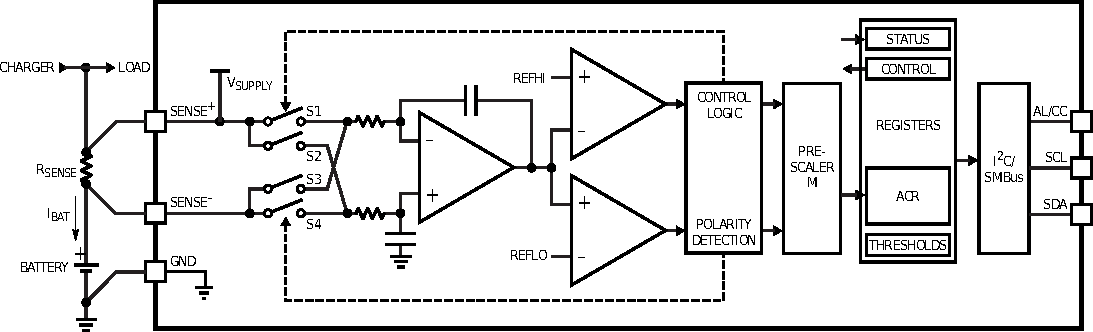
\includegraphics[width=\textwidth]{img/LTC2941-block}
    \end{center}
    \caption{blokové schéma obvodu LTC2941, převzato z katalogového listu výrobce}
\end{figure}
Použil jsem integrovaný obvod LTC2941 firmy Linear Technology. Tento obvod je stále připojený k akumulátoru přes snímací rezistor malé hodnoty, ze kterého v klidu odebírá proud pod $100~\jedn{\mu A}$.

Obvod v pravidelných časových okamžicích měří napětí na snímacím rezistoru a z jeho polarity určuje, jestli je akumulátor nabíjen či vybíjen a z hodnoty napětí a známého času měření dopočítává náboj.

Obvod je vybaven I2C sběrnicí, takže je velmi snadné z něj vyčítat informace o náboji v systému.

\section{Topologie napájecího systému}
\begin{figure}[H]
    \begin{center}
        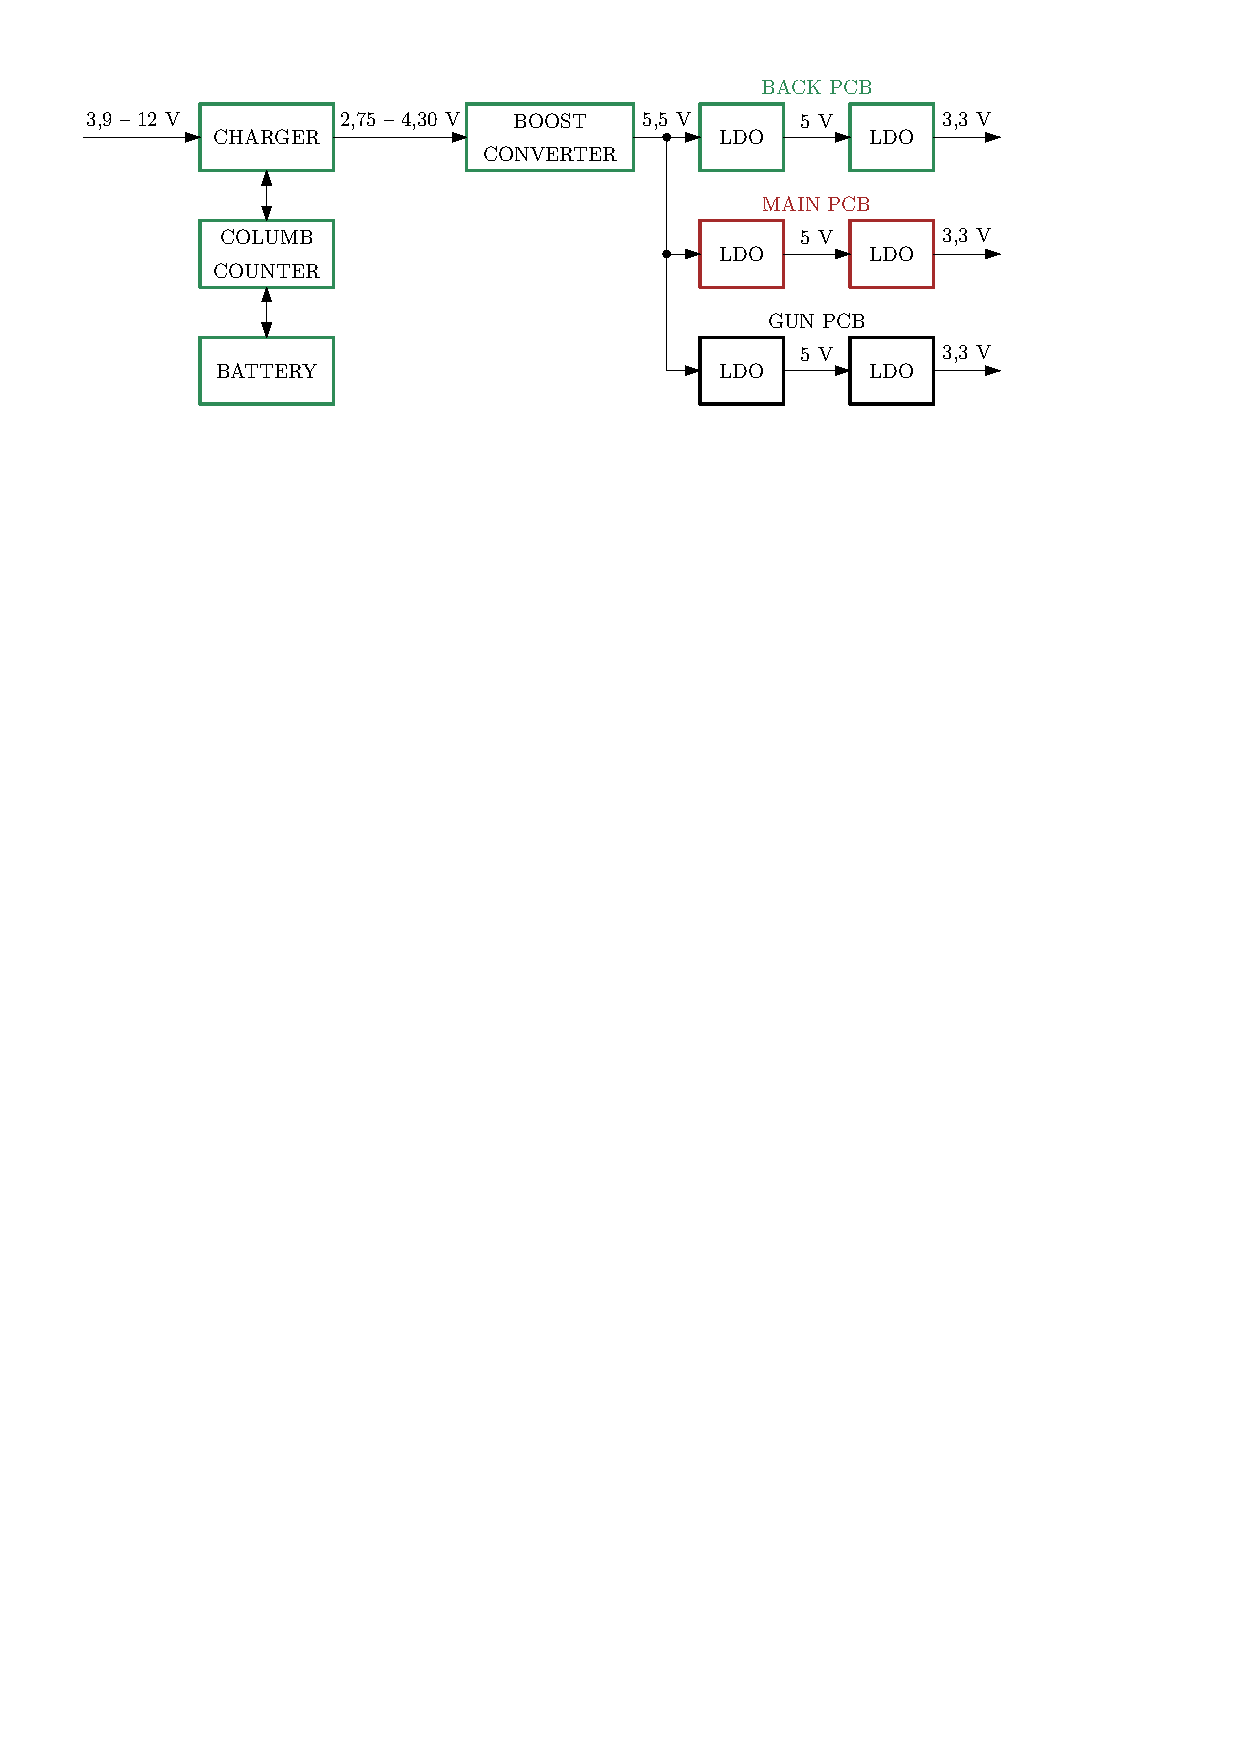
\includegraphics[width=\textwidth]{img/power-system}
    \end{center}
    \caption{blokové schéma napájecího systému}
\end{figure}

Většina bloků napájecího systému se nachází na plošném spoji (PCB) pojmenovaném back, který je umístěn na zádech hráče. Ten obstarává monitorování náboje, nabíjení akumulátoru a zvyšování napětí akumulátoru. Do všech částí vesty je přiváděno napětí 5,5~\jedn{V}, které je na výstupu zvyšujícího měniče. Poté je napětí snižováno pomocí nízko-úbytkových stabilizátorů (LDO).
